\chapter{Geoestatística utilizando o GSLib} 

\section{Introdução}

O GSLIB (Geostatistical Software Library) é um pacote de programas desenvolvidos em linguagem Fortran junto à Universidade de Stanford, nos Estados Unidos da América, sob a direção do professor André G. Journel e do professor Calyton V. Deutsch. Atualmente os pacotes de geoestatística para o GSLIB90 estão disponíveis no link \url{http://www.gslib.com/}, na aba Download. Além dos executáveis, é possível também baixar os códigos fontes em Fortran para cada um dos programas. 

Apesar de ser voltado principalmente para alunos de pós-graduação e pesquisadores, por ser um software gratuito muitas empresas ainda utilizam suas rotinas para análise geoestatística. O GSLIB pode ser considerado um dos melhores programas à disposição para análise espacial, permitindo o uso de algoritmos em diversas áreas como variografia, krigagem e simulação. Os resultados gráficos gerados pelo GSLIB são convertidos em arquivos PostScript. Para  a visualização e impressão dos dados podemos utilizar o programa Ghostscript obtido no link  \url{https://www.ghostscript.com/}. Outro programa importante para a visualização é o ghostviewer e pode ser obtido no seguinte link \url{http://www.ghostgum.com.au/software/gsview.htm}.

O GSLIB geralmente não se apresenta de forma amigável para o usuário pois são baseados em antigas plataformas como o DOS para windows, e não possuem uma interface gráfica. 

\section{A execução do GSLIB} 

Para rodar o GSLIb é necessário possuir os arquivos executáveis(.exe) em uma pasta no computador. Quando executado, o arquivo requisitará a criação de um arquivo (.par) na mesma pasta. Enquanto o arquivo executável é responsável pela execução do programa, o arquivo par é responsável por inserir os parâmetros necessários para o algoritmo. 

\section{Entrada de dados} \label{Arquivos_GSLIB}

Os dados de entrada do GSLIB são escritos em arquivos ASCII em um formato simplificado. Por convenção, os dados orientados para Leste são considerados no eixo X positivamente, enquanto os dados orientados para o Norte são considerados no eixo Y positivamente. Um banco de dados geoestatístico deve possuir a orientação da coordenada da amostra juntamente com o valor dos atributos associados. A seguir é demonstrado um exemplo de banco de dados do Walker Lake. Primeiramente informamos o nome do banco de dados, sem seguida o número de variáveis totais no banco, então fornecemos o nome de cada variável em cada linha e por último os dados são fornecidos em cada linha, separados com espaços. Para o funcionamento correto do GSLIB é necessário que a separação de decimais dos valores seja realizada por ponto. Os programas do GSLIB permitem a filtragem de valores faltantes. Isso pode ser feito dentro do arquivo par pelo método trimming limits. Como a filtragem é realizada nos extremos dos dados geralmente  se atribui um valor negativo muito grande como -999, filtrando apenas os valores acima de 0. É importante também remover quaisquer linhas no final do banco de dados vazia. 

\begin{small}
\begingroup
\inputencoding{ansinew}
\verbatiminput{./txt_files/walker_data.txt}
\endgroup
\end{small}

\section{Exemplos de aplicação do GSLIB} 

A seguir realizaremos alguns exemplos do uso do GSLIB no banco de dados do Walker Lake. O banco de dados apresenta coordenadas planas X e Y e mais duas variáveis de teor de cobre e ouro artificialmente criadas a partir de um banco de dados de topografia, de uma região de Nevada no Canadá. 

\subsection{Criando um histograma com o HISTPLT}

Para gerar o histograma utilizamos o programa HISTPLTt. O texto a seguir demonstra o arquivo de parâmetros. 

\begin{small} 
\begingroup
\inputencoding{ansinew}
\verbatiminput{./txt_files/hist_Cu.txt}
\endgroup
\end{small}
 
 Cada linha representa os seguintes parâmetros do arquivo de parâmetros.
 
\FloatBarrier 
\begin{enumerate}
	\item Endereço do arquivo do banco de dados 
	\item Número da coluna da esquerda para direita da variável e dos pesos para a geração do histograma 
	\item Limites para o uso dos dados. Limite inferior (-1.0) e limite superior ($10 ^{21} $)
	\item Nome do arquivo postscript de saída do histograma 
	\item Número mínimo e máximo demonstrado no histograma 
	\item Máxima frequência 
	\item Número de classes do histograma 
	\item Escala aritmética ou logarítmica 
	\item Histogramas de frequência ou acumulado 
	\item Número de quantis para o histograma acumulado 
	\item Número de decimais 
	\item Título do gráfico 
	\item posicionamento das estatísticas (-1 esquerda, 1 direita)
	\item ponto de referência para plotagem do gráfico de caixa 
\end{enumerate}
\FloatBarrier 


As figuras \ref{hist_walk_Cu_GSLIB} e \ref{hist_walk_Au_GSLIB} representam os histogramas das variáveis cobre e ouro. Podemos notar a assimetria característica das duas variáveis, principalmente na de ouro.

\FloatBarrier
\begin{figure}[h]
	\centering
	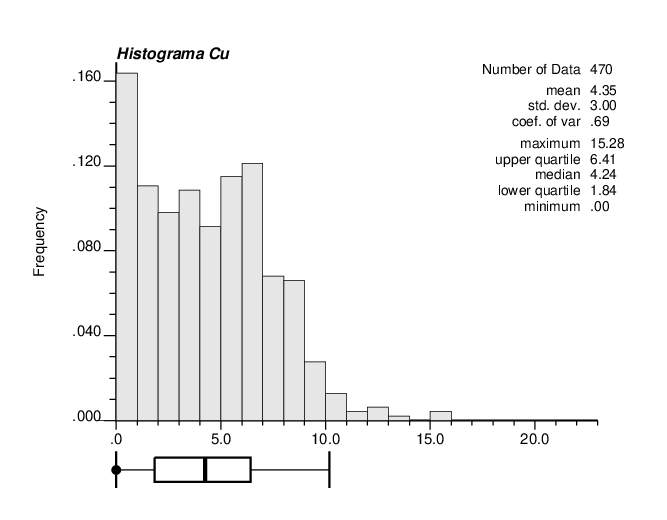
\includegraphics[scale=0.6]{./Capitulo_11/histograma_Cu.png}	
	\caption{ Histograma do Cobre para o depósito do Walker Lake}
	\label{hist_walk_Cu_GSLIB}
\end{figure}
\FloatBarrier


\FloatBarrier
\begin{figure}[h]
	\centering
	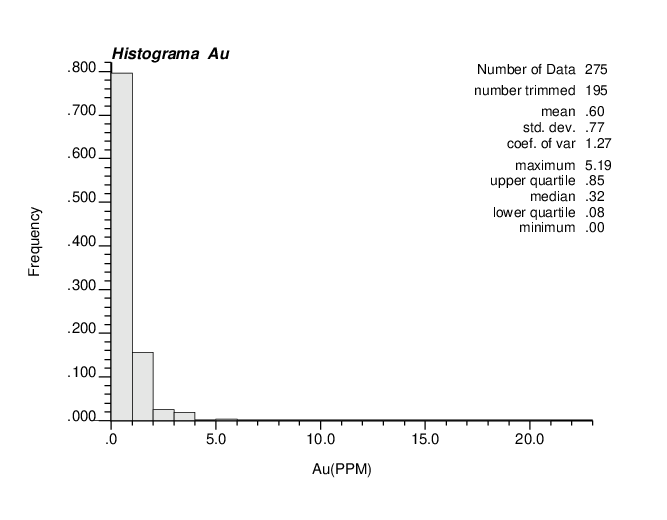
\includegraphics[scale=0.6]{./Capitulo_11/histograma_Au.png}	
	\caption{ Histograma do Ouro para o depósito do Walker Lake}
	\label{hist_walk_Au_GSLIB}
\end{figure}
\FloatBarrier

\subsection{Criando um gráfico de dispersão com o SCATPLT}

Gráficos de dispersão são uma boa forma de se avaliar a dependência entre duas variáveis X e Y diferentes. Para realizar o gráfico de dispersão é demonstrado a seguir o arquivo de parâmetros utilizado no depósito Walker Lake do programa SCATPLT. 

\FloatBarrier 
\begingroup
\inputencoding{ansinew}
\verbatiminput{./txt_files/scatplt.txt}
\endgroup
\FloatBarrier

Em seguida é demonstrado o significado de cada parâmetro no arquivo .par. 

\begin{enumerate}
	\item Endereço do arquivo do banco de dados 
	\item Número da coluna X, da coluna Y, os pesos de desagrupamento e uma terceira variável  
	\item Limites para o uso dos dados. Limite inferior (-1.0) e limite superior ($10 ^{21} $)
	\item Nome do arquivo postscript de saída do histograma 
	\item Número mínimo, máximo da variável X e escolha da escala (0 = aritmética, 1 = logarítmica)
	\item Número mínimo, máximo da variável Y e escolha da escala (0 = aritmética, 1 = logarítmica)
	\item Plotar a cada n pontos 
	\item Tamanho do ponto no gráfico 
	\item Limites para a terceira variável 
	\item Título do gráfico
\end{enumerate}
\FloatBarrier

A figura \ref{dispersao_GSLIB} demonstra o resultado para as variáveis cobre e ouro do depósito Walker Lake. Nota-se que o coeficiente de correlação de Pearson é baixo, apresentando valor de 0.551. Também é apresentado na figura o coeficiente de rank de 0.762, demonstrando que pode haver uma correlação não necessariamente linear entre as variáveis. 

\FloatBarrier
\begin{figure}[h]
	\centering
	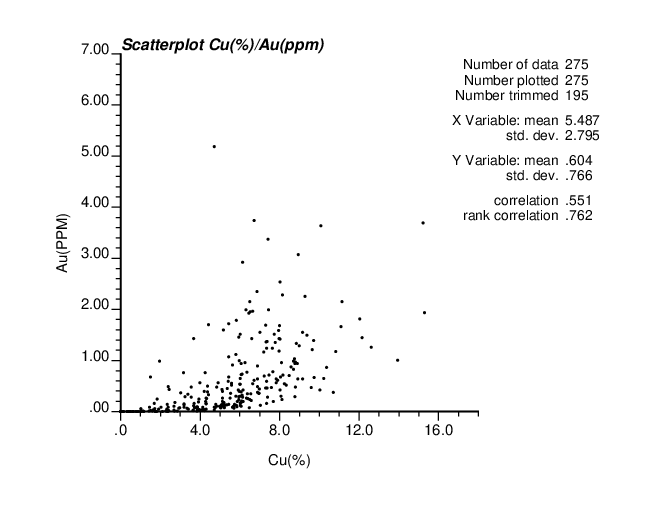
\includegraphics[scale=0.6]{./Capitulo_11/scatplt.png}	
	\caption{ Diagrama de dipersão do Cobre e Ouro para o depósito do Walker Lake}
	\label{dispersao_GSLIB}
\end{figure}
\FloatBarrier

\subsection{Criando um mapa de localização com o LOCMAP}

Os mapas de localização são uma forma visual interessante para se determinar os padrões de localização das amostras, tal como as regiões onde ocorrem anomalias positivas e negativas. A seguir é demonstrado o arquivo de parâmetros do arquivo .par do programa LOCMAP. 

\begin{small}
\begingroup
\inputencoding{ansinew}
\verbatiminput{./txt_files/locmap_cu.txt}
\endgroup
\end{small}

Em seguida são demonstrados os significados dos parâmetros em cada linha do arquivo .par.

\begin{enumerate}
	\item Endereço do arquivo do banco de dados 
	\item Número da coluna X, da coluna Y, os pesos de desagrupamento e uma terceira variável  
	\item Limites para o uso dos dados. Limite inferior (-1.0) e limite superior ($10 ^{21} $)
	\item Nome do arquivo postscript de saída do histograma 
	\item Número mínimo, máximo da variável X 
	\item Número mínimo, máximo da variável Y 
	\item Plotar os valores dos dados ou da validação cruzada (0=dados, 1=validação cruzada)
	\item Plotar dados em escala aritmética ou logarítmica (0=aritmética, 1=logarítmica)
	\item Escala de cor cinza ou colorida (0=cinza, 1= colorida)
	\item adição de rótulos nos dados (0= sem rótulos, 1= rótulo dos dados)
	\item valor mínimo, máximo e incremento da escala 
	\item tamanho da fonte dos rótulos
	\item Título do gráfico
\end{enumerate}

A figura \ref{scatplot_gslib} demonstra o resultado gráfico do mapa de localização das amostras do Walker Lake. Podemos notar um corpo de maior extensão no flanco oeste e corpos menores ao leste. A orientação do corpo maior possui alongamento na direção sudeste. Os valores mais intensos de teor de cobre se encontram dentro do corpo geológico, enquanto as bordas se apresentam mais pobres.
 
\FloatBarrier
\begin{figure}[h]
	\centering
	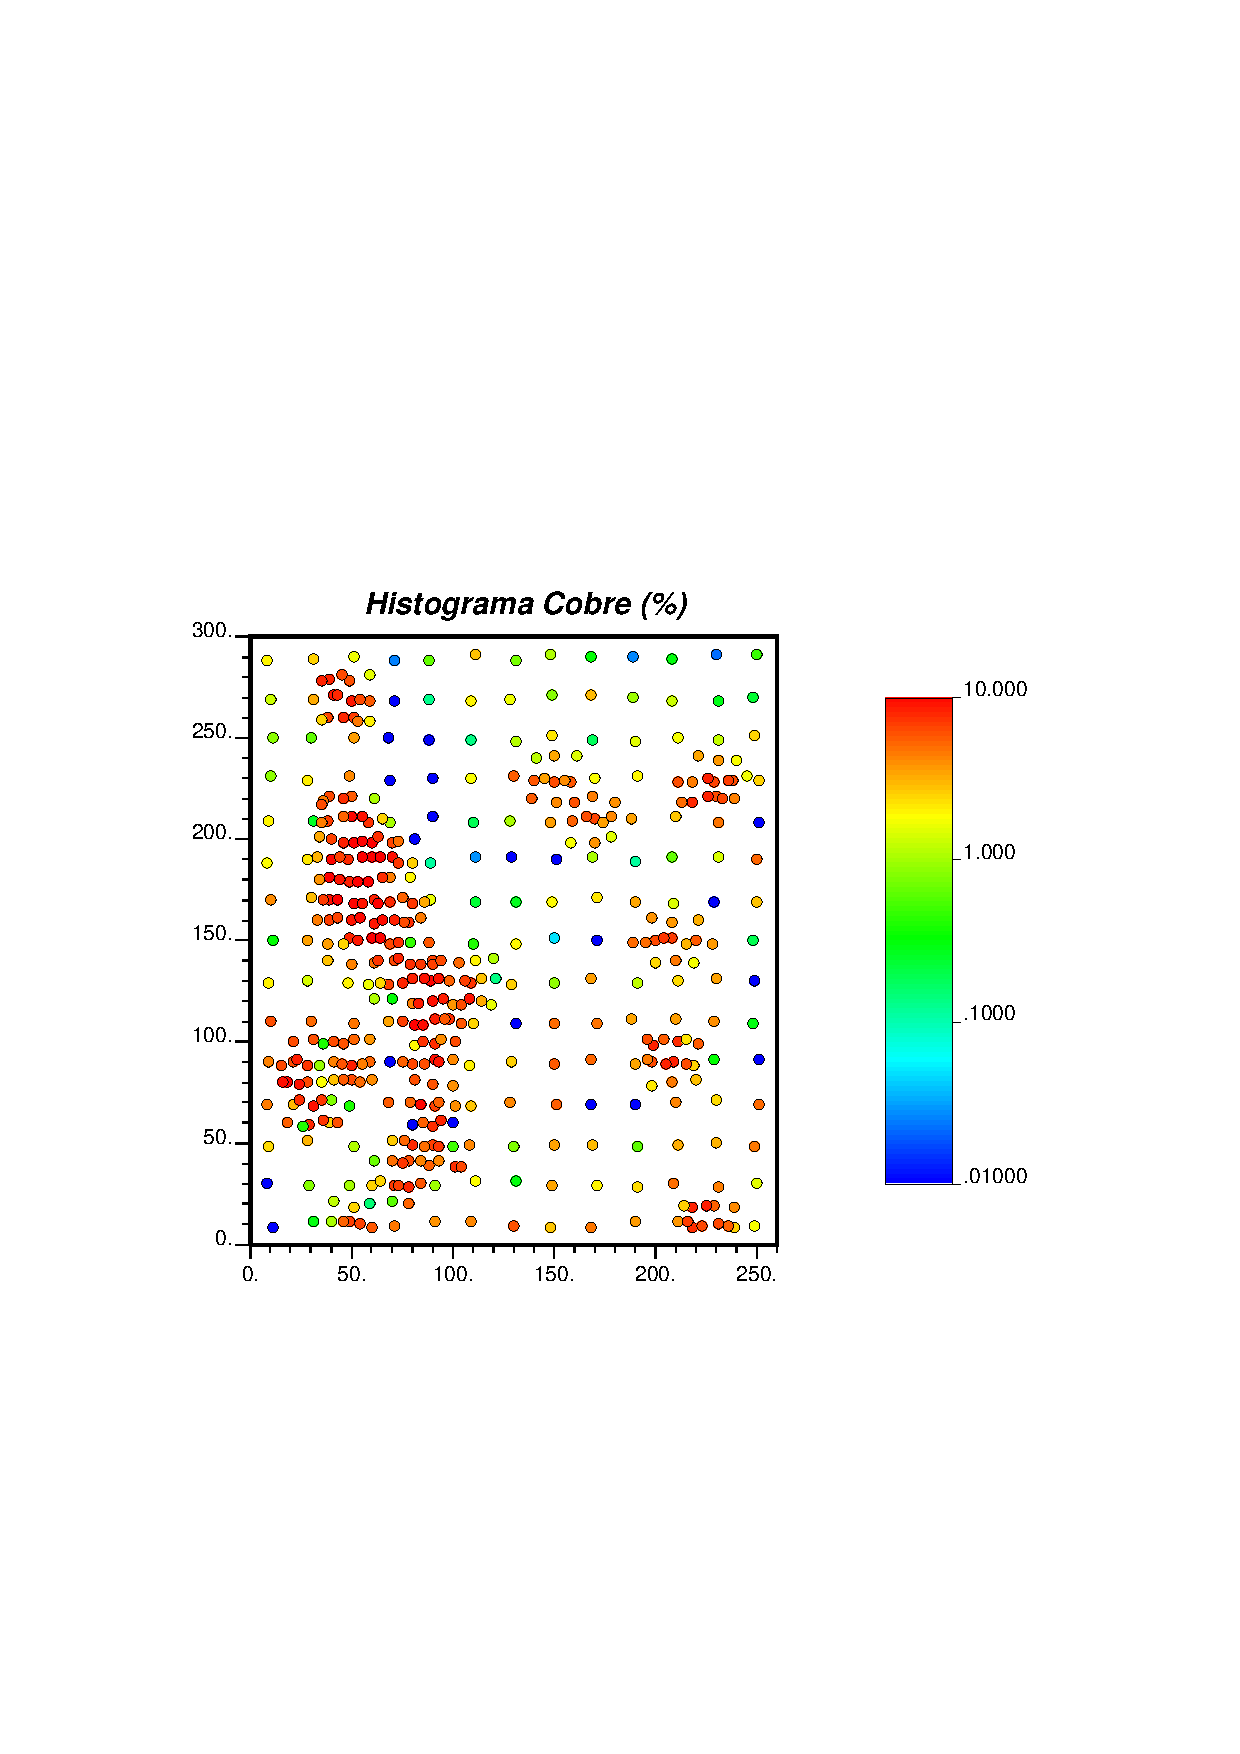
\includegraphics[scale=0.7]{./Capitulo_11/Mapa_Cu.png}	
	\caption{ Mapa de localização da variável cobre para o depósito do Walker Lake}
	\label{scatplot_gslib}
\end{figure}
\FloatBarrier

\section{desagrupamento utilizando células móveis com o DECLUS}

Para comparar as estatísticas interpoladas com as estatísticas dos dados é necessário utilizar alguma técnica de desagrupamento. O GSLIB permite realizar o desagrupamento a partir de céclulas móveis utilizando o programa DECLUS. Em seguida demonstramos o arquivo de parâmetros do programa.

\begin{small}
	\begingroup
	\inputencoding{ansinew}
	\verbatiminput{./txt_files/declus.txt}
	\endgroup
\end{small}

Em seguida são demonstrados os significados dos parâmetros em cada linha do arquivo .par.

\begin{enumerate}
	\item Endereço do arquivo do banco de dados 
	\item Colunas para a variável X, Y, Z e a variável desagrupada 
	\item Limites para o uso dos dados. Limite inferior ($-10 ^{21} $) e limite superior ($10 ^{21} $)
	\item Nome do arquivo de sumário estatístico do desagrupamento 
	\item Nome do arquivo de saída com os resultados e o peso de cada amostra
	\item Anisotropia da célula na direção Y e em Z. (Tamanho em y = tamanho* yanisotropia)
	\item Procurar pela valor mínimo da média (0=mínimo, 1=máximo)
	\item Número de células para o desagrupamento, os tamanhos mínimos e máximos da célula
	\item Tamanho aumentado de cada célula. Essa medida evita com que valores na borda das células tenham problemas.
\end{enumerate}

Podemos realizar o histograma dos dados desagrupados utilizando o programa HISTPLT. Para gerar o gráfico com os pesos basta apenas colocar na segunda linha a coluna dos pesos de desagrupamento do arquivo declus.out. 

\FloatBarrier
\begin{figure}[h]
	\centering
	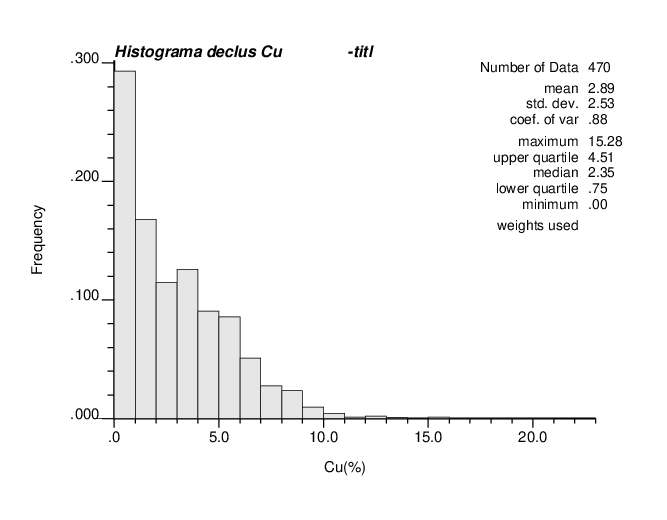
\includegraphics[scale=0.6]{./Capitulo_11/declus.png}	
	\caption{ Histograma dos dados desagrupados pelo GSLIB}
	\label{declus}
\end{figure}
\FloatBarrier

\section{Convenção da orientação de eixos de anisotropia do GSLIB} \label{orient}

O GSLIB possui uma convenção própria de orientação dos eixos para a modelagem variográfica. A direção principal da continuidade espacial é orientada segundo o eixo Y inicialmente. A figura \ref{alinhamento} demonstra este alinhamento dos eixos. 

\FloatBarrier
\begin{figure}[h]
	\centering
	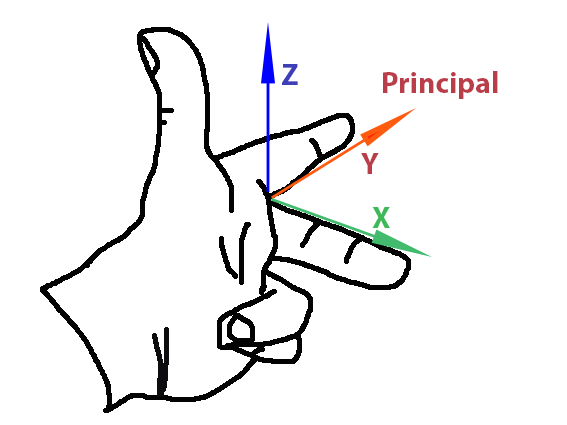
\includegraphics[scale=0.2]{./Capitulo_11/Direcao_mao.png}	
	\caption{ Alinhamento inicial dos eixos do variograma segundo a notação do GSLIB}
	\label{alinhamento}
\end{figure}
\FloatBarrier

As rotações podem ser realizadas no sentido horário e anti-horário segundo este eixo de referência. A figura \ref{Orientacao} demonstra o sentido positivo e negativo de rotação dos eixos segundo a notação do GSLIB. 

\FloatBarrier
\begin{figure}[h]
	\centering
	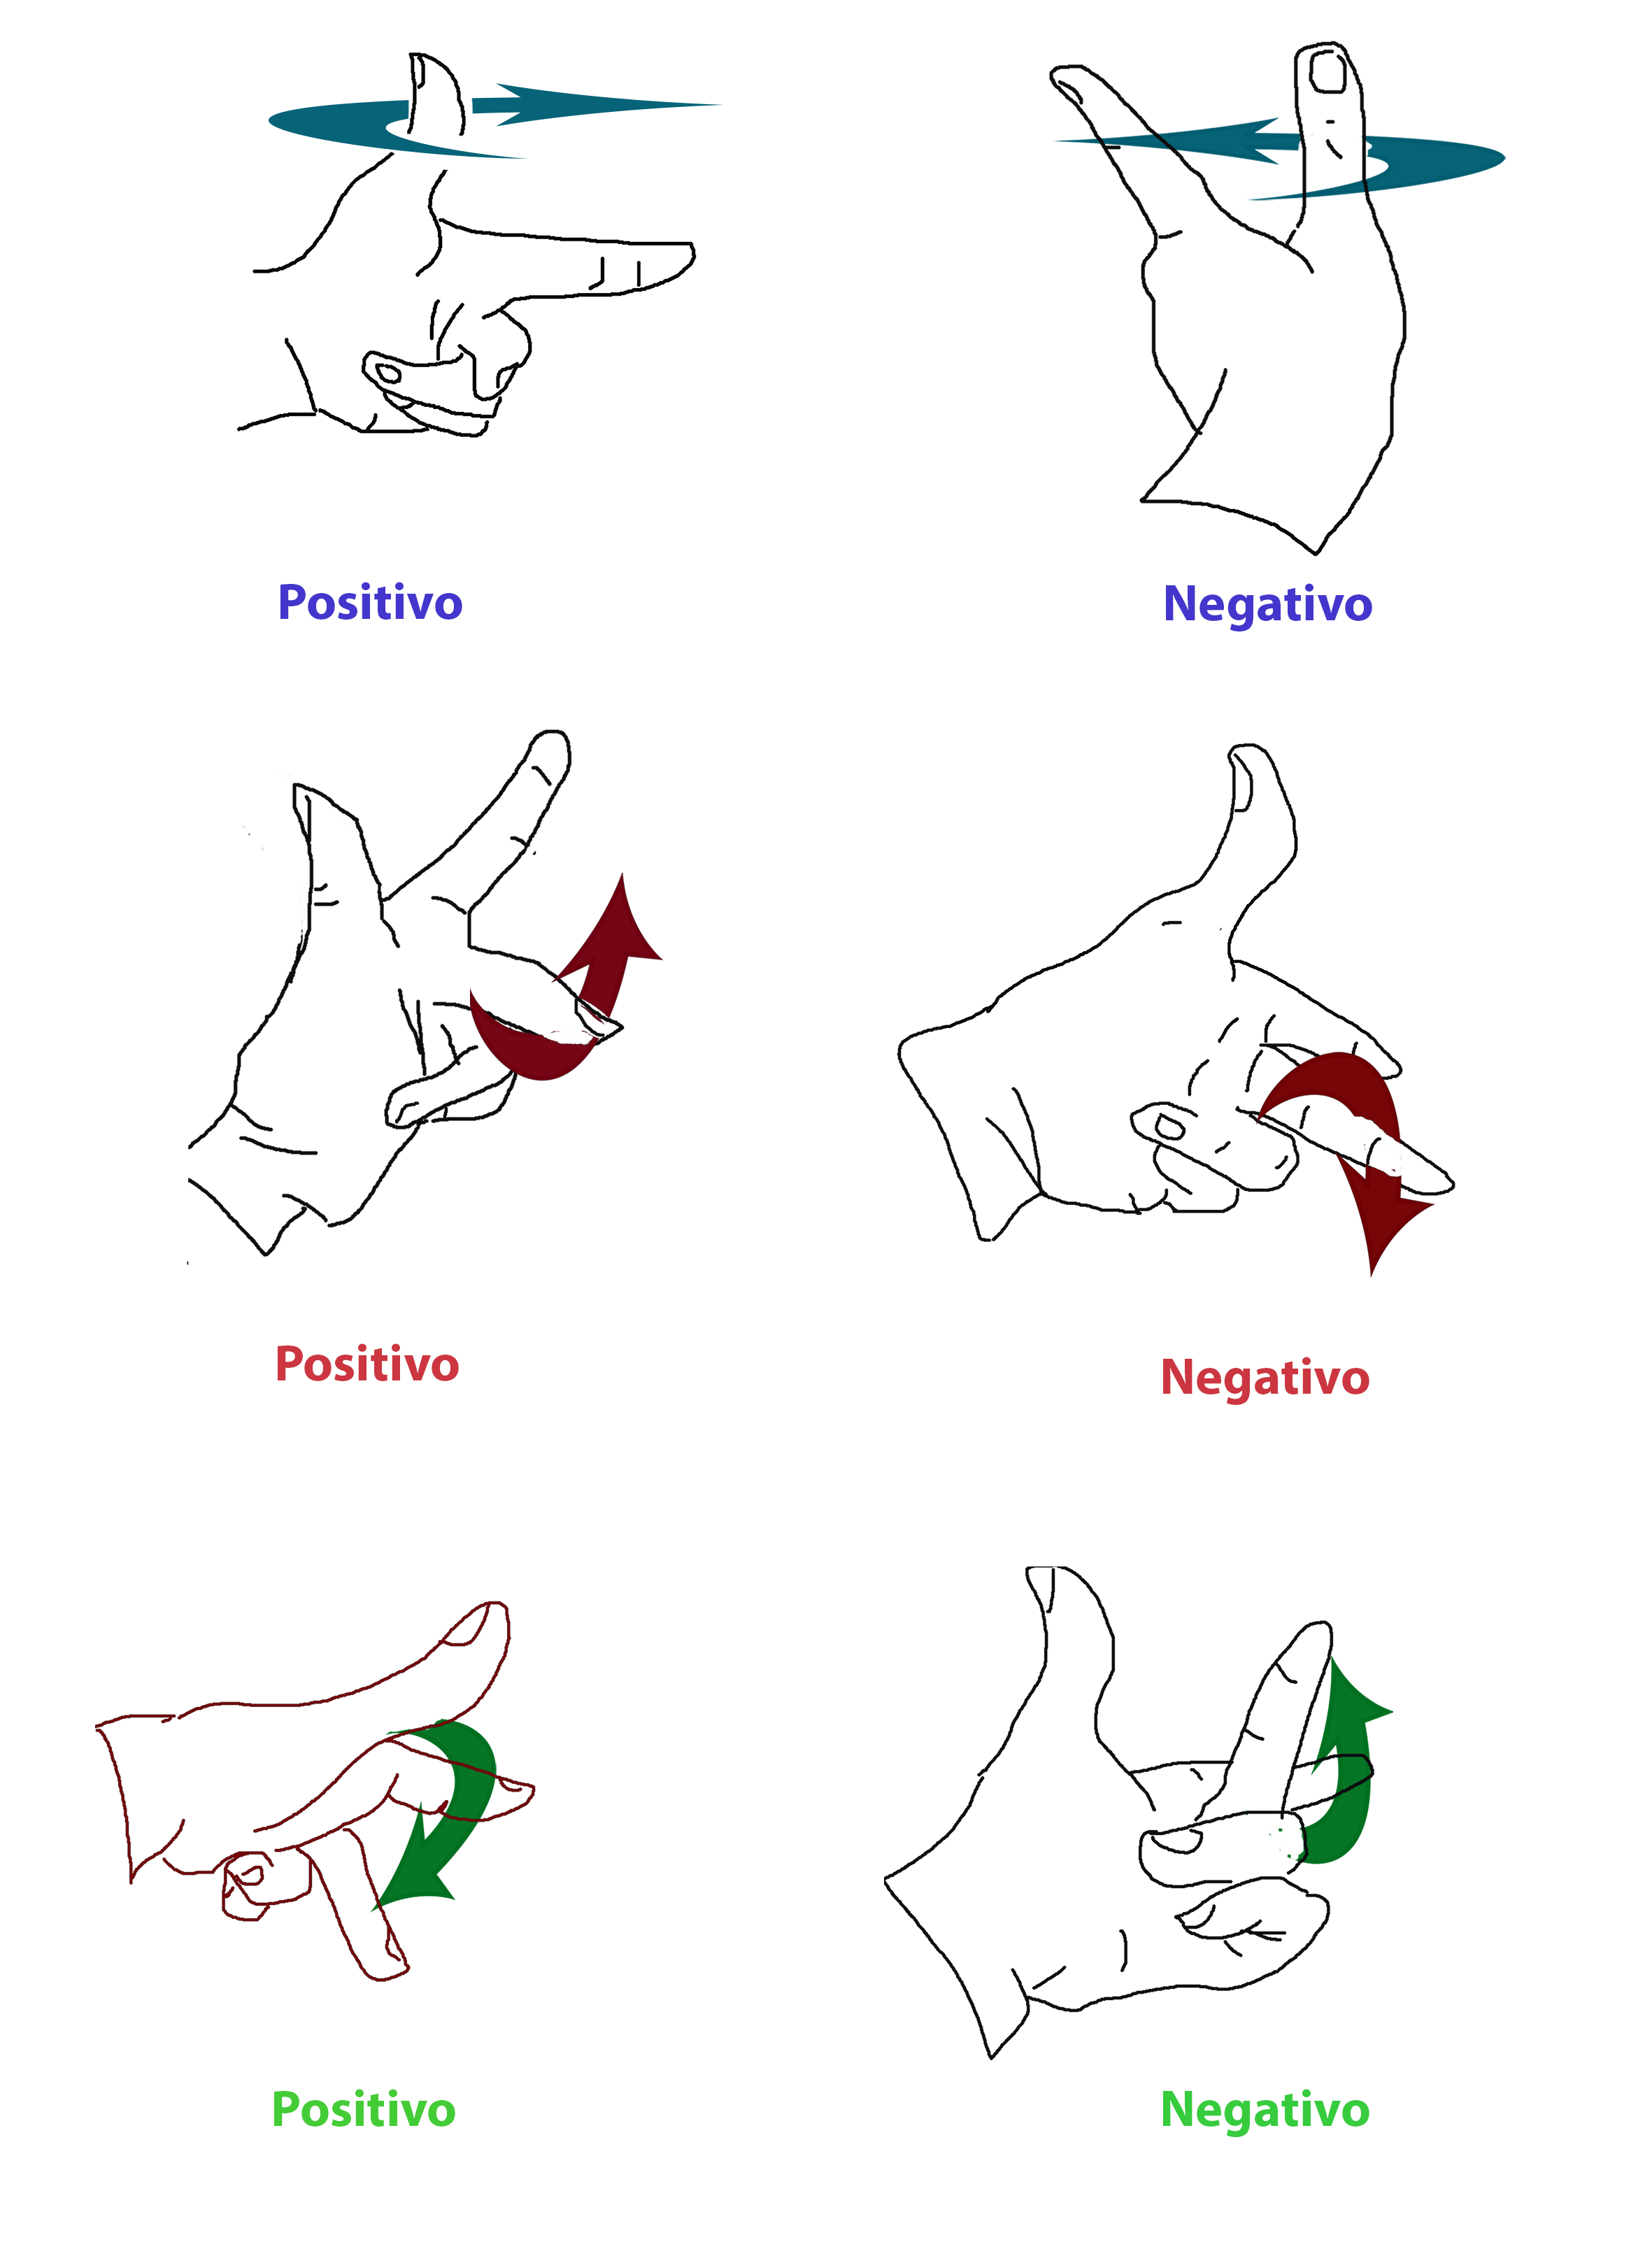
\includegraphics[scale=0.6]{./Capitulo_11/Orientacao_gslib.png}	
	\caption{ Orientação dos eixos do variograma segundo a notação do GSLIB}
	\label{Orientacao}
\end{figure}
\FloatBarrier

\section{Variograma experimental (GAMV/ VARGPLT) }

Variogramas experimentais podem ser facilmente criados com o programa GAMV. Além das funções tradicionais de variograma e covariograma, o programa também permite diversos outros tipos de funções como as funções pairwise, semimadograma e semivariograma de logaritmos. A seguir é demonstrado o arquivo .par para os variogramas experimentais de cobre do depósito Walker Lake.

\begin{small}
	\begingroup
	\inputencoding{ansinew}
	\verbatiminput{./txt_files/gamv.txt}
	\endgroup
\end{small}

A seguir é demonstrado o significado do arquivo de parâmetros do GamV. É necessário que as informações descritas no arquivo de parâmetros sejam compatíveis, pois caso houver discrepâncias o programa envia uma mensagem de erro. O número de direções fornecidas, por exemplo, deve ser o mesmo do número de linhas contendo os parâmetros de azimute, mergulho, etc. O número de variáveis e o número das colunas relativas a cada uma destas variáveis também deve ser o mesmo. 

\begin{enumerate}
	\item Endereço do arquivo do banco de dados 
	\item Número da coluna X, Y e Z
	\item Número de variáveis utilizadas e número das colunas 
	\item Limites para o uso dos dados. Limite inferior ($-10 ^{21}$) e limite superior ($10 ^{21} $)
	\item Número de lags utilizados no variograma (distância = número do lag* tamanho do lag)
	\item Tamanho do lag 
	\item Número de direções 
	\item Orientação : azimute, tolerância horizontal, banda horizontal, mergulho, tolerância vertical, banda vertical
	\item Normalização do patarmar 
	\item Número de variogramas 
	\item variável da extermidade superior do vetor, variável da extremidade inferior do vetor e o tipo do variograma
\end{enumerate}

Para realizar a plotagem do gráfico é necessário outro programa chamado de VARGPLT. Este programa gera o arquivo .ps contendo a imagem dos variogramas experimentais.

\begin{small}
	\begingroup
	\inputencoding{ansinew}
	\verbatiminput{./txt_files/varplot_exp.txt}
	\endgroup
\end{small}

A seguir encontra-se a explicação de cada um dos parâmetros do arquivo. Lembre-se que antes de informar cada variograma é necessário colocar o arquivo de entrada do variograma experimental.

\begin{enumerate}
	\item Nome do arquivo de saída PostScript (.ps)
	\item Número de variogramas para plotagem (Um para cada direção e modelo)
	\item Distância mínima e máxima do variograma experimental
	\item Valor mínimo e máximo do variograma experimental 
	\item Plotagem do sill e o seu valor (0= não plotar, 1=plotar)
	\item Título do variograma experimental 
	\item Arquivo contendo os dados do variograma experimental 
	\item Número do variograma, e parâmetros estéticos
\end{enumerate}

O resultado dos variogramas podem ser vistos na figura \ref{Variograma experimntal}, onde a curva vermelha representa a direção de maior continuidade (Azimute = 157.5 graus )e a curva azul representa a direção de menor continuidade espacial (Azimute = 67.5 graus).

\FloatBarrier
\begin{figure}[h]
	\centering
	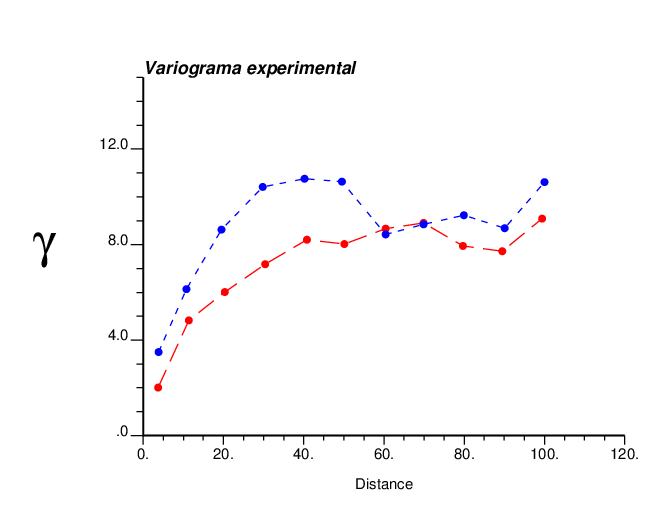
\includegraphics[scale=0.6]{./Capitulo_11/experimentais.png}	
	\caption{ Variogramas experimentais do Walker Lake. Curva vermelha representando a maior continuidade no azimute de 157.5 graus e curva preta representando a menor continuidade no azimute 67.5 graus norte.}
	\label{Variograma experimntal}
\end{figure}
\FloatBarrier

\section{Modelagem de variogramas (VMODEL/VARGPLT) }

Para criar modelos de variograma podemos utilizar o programa VMODEL para gerar um arquivo com a curva modelada. A seguir é demonstrado o arquivo de parâmetros do programa. 

\begin{small}
	\begingroup
	\inputencoding{ansinew}
	\verbatiminput{./txt_files/Vmodel.txt}
	\endgroup
\end{small}

O GSLIB apresenta três tipos de modelos de continuidade espacial definidos por números. O tipo do variograma pode ser especificado de acordo com a seguinte lista

\begin{enumerate}
	\item Variograma esférico 
	\item Variograma exponencial 
	\item Variograma gaussiano 
\end{enumerate}

A seguir encontra-se a explicação de cada um dos parâmetros do arquivo. Lembre-se que as informações fornecidas no arquivo devem ser compatíveis para que não ocorra erro na execução do programa. O número de direções fornecidas, por exemplo, deve ser o mesmo que o número de linhas contendo as informações do azimute e mergulho. 

\begin{enumerate}
	\item Nome do arquivo de saída do modelo de variograma 
	\item Número de direções e número de lags utilizados.
	\item Para cada direção o azimute, mergulho e tamanho do lag 
	\item Número de estruturas e efeito pepita 
	\item Para cada estrutura o tipo do variograma, a contribuição, e os ângulos de rotação segundo a convenção GSLIB. (ang1 = rotação de Z, ang2 = rotação de X, ang3= rotação de Y). Para mais informações veja na seção \ref{orient} a orientação dos eixos de anisotropia
	\item Alcance na direção principal (orientada em Y inicialmente), alcance na direção mínima (orientada em X inicialmente) e alcance na direção vertical (orientada em Z inicialmente)
\end{enumerate}

Para gerar o arquivo dos modelos de variograma juntamente com os dados experimentais, modificamos o arquivo VARGPLT anterior adicionando os dois variogramas a mais e modificando o número de variogramas plotados.

\begin{small}
	\begingroup
	\inputencoding{ansinew}
	\verbatiminput{./txt_files/model.txt}
	\endgroup
\end{small}

A figura \ref{modelo_var} representa o ajuste do variograma para a variável cobre no depósito Walker Lake.

\FloatBarrier
\begin{figure}[h]
	\centering
	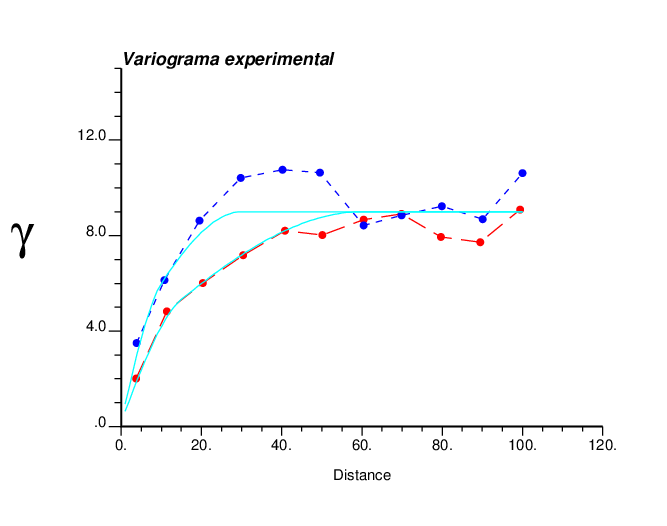
\includegraphics[scale=0.6]{./Capitulo_11/model.png}	
	\caption{ Modelo de variograma com duas estruturas para o Walker Lake. Curva vermelha representando a maior continuidade no azimute de 157.5 graus e curva preta representando a menor continuidade no azimute 67.5 graus norte. Curva azul claro representado o modelo.}
	\label{modelo_var}
\end{figure}
\FloatBarrier

\section{Validação Cruzada com (KT3D/LOCMAP)}

Para ajustar a melhor estratégia de busca das amostras na krigagem, bem como também ajustar o melhor modelo de variograma, podemos utilizar a validação cruzada como uma alternativa para identificar os possíveis erros de estimativa. A seguir é demonstrado o arquivo de parâmetros do programa KT3D utilizado não apenas para a validação cruzada, mas também para a krigagem. O programa KT3D não apenas realiza krigagem ordinária, mas diversos outros tipos de krigagem. Neste exemplo realizaremos apenas a krigagem ordinária. Em dados tridimensionais uma alternativa mais interessante que a validação cruzada é o jacknife, em que furos são retirados como um todo e os erros computados em cada um deles. Como nos casos tridimensionais as compostas são muito próximas uma das outras, os erros de validação cruzada tendem a ser muito pequenos, falseando um melhor ajuste dos dados. 


\begin{small}
	\begingroup
	\inputencoding{ansinew}
	\verbatiminput{./txt_files/kt3d_cross.txt}
	\endgroup
\end{small}

A seguir encontra-se a explicação de cada um dos parâmetros do arquivo.

\begin{enumerate}
	\item Arquivo contendo os dados 
	\item colunas para o índice do furo, coordenas X,Y,Z a variável de interesse e uma variável secundária
	\item Limites para o uso dos dados. Limite inferior ($-10 ^{21}$) e limite superior ($10 ^{21} $)
	\item Opções da krigagem (0= em malha, 1= validação cruzada, 2= jacknife). Marque 1 para realizar a validação cruzada.
	\item arquivo para utilização do jacknife. Caso não exista este arquivo o programa simplesmente ignora esta instrução.
	\item Variável X, Y, Z a variável de interesse e a variável secundária. Adicione 0 caso não possua esta informação em algum tópico. Por exemplo em casos 2D utilizamos a coordenada Z = 0.
	\item Nível de depuração da krigagem. Quanto maior o nível de depuração, maiores serão as informações contidas no arquivo de depuração .dgb. Para um nível 3 de depuração é possível verificar as matrizes de krigagem e dados utilizados no cálculo. 
	\item Nome do arquivo de depuração
	\item Nome do arquivo de saída da krigagem 
	\item número de células em X, o valor mínimo do grid em X e o tamanho da célula em X
	\item número de células em Y, o valor mínimo do grid em Y e o tamanho da célula em Y
	\item número de células em Z, o valor mínimo do grid em Z e o tamanho da célula em Z
	\item Discretização dos blocos da krigagem em x, y e z para krigagem de blocos.
	\item Número mínimo de dados utilizados e número máximo.
	\item Máximo número de dados por octante. (0 para não ser utilizado)
	\item Tamanho dos eixos de anisotropia para a estratégia de busca. Tamanho na direção principal, tamanho na direção mínima e tamanho na direção vertical.
	\item Ângulos de rotação do elipsóide de anisotropia segundo a convenção GSLIB. Rotação no eixo Z, rotação no eixo X e rotação no eixo Y. Verificar na seção \ref{orient} a conveção do programa. 
	\item Escolha do tipo de krigagem (0 = krigagem simples, 1= krigagem ordinária, 2= krigagem não estacionária, 3= krigagem com tendência externa) e o valor médio caso seja selecionada a krigagem simples. Em outros casos o programa ignora este parâmetro. 
	\item Coeficiente dos polinômios em caso de krigagem não estacionária. 
	\item Estimativa da variável ou da tendência (0= variável, 1= tendência)
	\item Arquivo com tendência externa caso seja realizada krigagem com tendência externa.
	\item Coluna da tendência no arquivo
	\item Adição dos variogramas: Número de estruturas e efeito pepita 
	\item Para cada estrutura p tipo do modelo de variograma, contribuição, rotação no eixo Z, rotação no eixo X e rotação no eixo Y segundo a referência do GSLIB. 
	\item Para cada estrutura os alcances na direção principal, mínima e vertical.
	
\end{enumerate}

Para a plotagem do mapa de validação cruzada podemos utilizar o arquivo LOCMAP lembrando sempre de marcar a opção de validação cruzada. A seguir é demonstrado o arquivo de parâmetros .par do programa LOCMAP. 

\begin{small}
	\begingroup
	\inputencoding{ansinew}
	\verbatiminput{./txt_files/locmap_cross.txt}
	\endgroup
\end{small}

A figura \ref{cruzado_gslib} demonstra o mapa da validação cruzada para a variável cobre no depósito Walker Lake. 

\FloatBarrier
\begin{figure}[h]
	\centering
	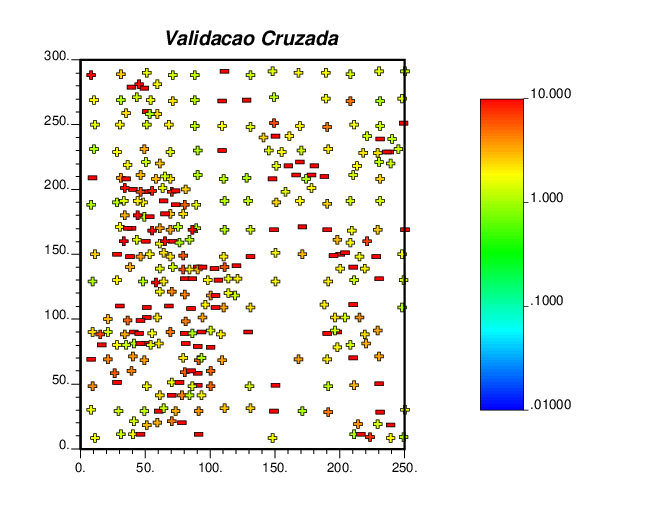
\includegraphics[scale=0.8]{./Capitulo_11/cruzado.png}	
	\caption{ Mapa da validação cruzada para a variável cobre, no depósito Walker Lake.}
	\label{cruzado_gslib}
\end{figure}
\FloatBarrier

\section{Krigagem com (KT3D/PIXELPLT)}

O arquivo de parâmetros para a krigagem é o mesmo que o utilizado para a validação cruzada, apenas alterando a opção de validação cruzada (1) para malha (0). A explicação dos parâmetros do arquivo pode ser obtida na seção anterior. A seguir é demonstrado o arquivo do tipo .par utilizado para a krigagem da variável cobre no depósito Walker Lake.  

\begin{small}
	\begingroup
	\inputencoding{ansinew}
	\verbatiminput{./txt_files/kt3d_krig.txt}
	\endgroup
\end{small}

Para a plotagem do mapa de krigagem utilizamos o programa PIXELPLT. A seguir é dmeonstrado o arquivo .par do programa.

\begin{small}
	\begingroup
	\inputencoding{ansinew}
	\verbatiminput{./txt_files/pixelplt.txt}
	\endgroup
\end{small} 

A explicação dos parâmetros do arquivo é demonstrada a seguir

\begin{enumerate}
	\item Nome do arquivo dos dados krigagdos 
	\item Coluna da variável a ser plotada 
	\item Limites para o uso dos dados. Limite inferior ($-10 ^{21}$) e limite superior ($10 ^{21} $)
	\item Nome do arquivo de saída .ps 
	\item Número de realizações. No caso de krigagem possuímos apenas uma realização. No entanto nos casos de simulação podem haver mais de uma realização.
	\item Número de células em X, valor mínimo da coordenada X e tamanho da célula e X
	\item Número de células em Y, valor mínimo da coordenada Y e tamanho da célula e Y  
	\item Número de células em Z, valor mínimo da coordenada Z e tamanho da célula e Z
	\item Orientação do corte realizado em malhas tridimensionais. (1=orientação horizontal XY, 2= Corte vertical em XZ, 3= Corte vertical em YZ)
	\item Número do corte 
	\item Título do gráfico
	\item Título da coordenada leste 
	\item Título da coordenada Norte 
	\item Escala aritmética ou logarítmica (0=aritmética, 1=logarítmica)
	\item Escala de cinza ou de cores (0=cinza, 1=de cores)
	\item Variável de entrada contínua ou categórica (0=contínua, 1=categórica)
	\item Número mínimo, máximo e incremento da variável plotada
	\item Número de categorias se selecionada variável categórica
	\item Categoria, cor e nome da categoria
\end{enumerate}

As figuras \ref{krigado_gslib} e \ref{krigado_var_gslib} demonstram os mapas krigados e a variância de krigagem para o depósito Walker Lake. 

\FloatBarrier
\begin{figure}[h]
	\centering
	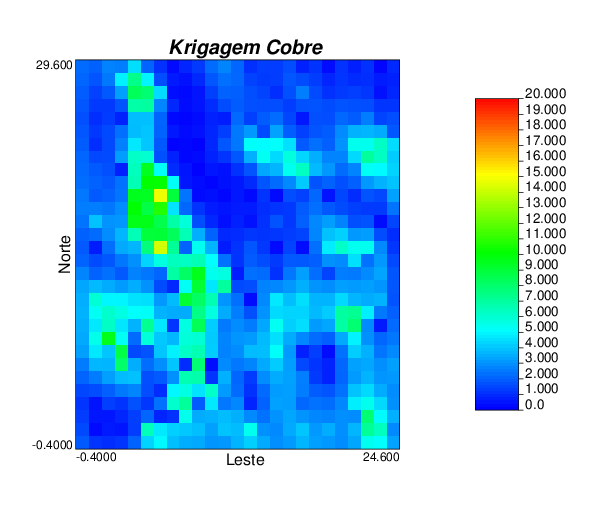
\includegraphics[scale=0.8]{./Capitulo_11/krigado.png}
	\caption{ Mapa da krigagem para a variável cobre, no depósito Walker Lake.}
	\label{krigado_gslib}
\end{figure}
\FloatBarrier

\FloatBarrier
\begin{figure}[h]
	\centering
	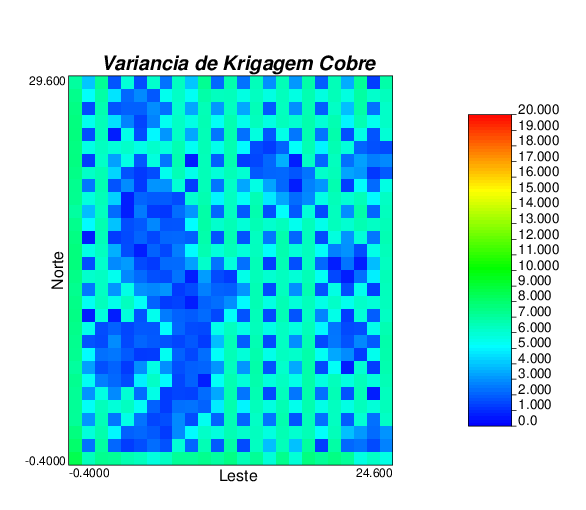
\includegraphics[scale=0.8]{./Capitulo_11/krigado_var.png}	
	\caption{ Mapa da variância de krigagem para a variável cobre, no depósito Walker Lake.}
	\label{krigado_var_gslib}
\end{figure}
\FloatBarrier
